Intuitively, we expect that objects within an image that are most salient are likely to be remembered, since they tend to draw a viewer's attention, i.e. a majority of his/her eye fixations will lie within those object regions. On the other hand, it is conceivable that some visually appealing regions will not be memorable, especially since aesthetic images are known to be less memorable \cite{isola11,isola14}. When can visual saliency predict object memorability and what are the possible differences between the two? Studying the relationship between saliency and memorability is paramount for understanding object memorability in greater depth.

\begin{figure}[t]
\centering
\subfigure{\centering \includegraphics[width=0.47\textwidth]{figures/results/fixation/fix_corr_set.png}}
\vspace{-5mm}\caption{\footnotesize\textbf{Correlations between memorability, fixation count, and number of objects.} Left: Memorability and fixation counts correlate positively. Middle:  Memorability and number of objects are negatively correlated. Right: Fixations and object counts are weakly negatively correlated.}\label{fig:scatterFixation}%\vspace{-12pt}
\end{figure}

To address this query, we utilize the eye fixation data made available for the Pascal-S dataset \cite{yin14}. First, we compute the number of unique fixation points within the image segment of each object and the correlation between this metric and the object's memorability score (refer to Figure \ref{fig:scatterFixation} (\emph{left})). We find this correlation to be positive and considerably high ($\rho = 0.71$), suggesting that fixation count and visual saliency may drive object memorability considerably. However, the large concentration of points on the bottom left part of the scatter plot in Figure \ref{fig:scatterFixation} (\emph{left}) suggests that part of the reason for this high correlation is that objects that have not been viewed (i.e. no fixation points associated with them) at all have essentially no memorability, and therefore will always imply correlation. If we remove these simple cases, we can examine whether or not the full range of memorability scores is predicted by fixation count. To investigate this, we plot the change in correlation between object memorability and fixations as the minimum number of fixations inside objects increases. For each minimum fixation count, we compute the memorability-fixation correlation again but \emph{only} using objects that contain at least this number of fixations (refer to Figure \ref{fig:fixCorr} (\emph{right})). The decreasing trend in correlation indicates that as the number of fixations inside an object increases, the predictive ability diminishes significantly, indicating that the full range of memorability scores are not well predicted. In addition, Figure \ref{fig:fixCorr} (\emph{left}) plots this correlation as a function of total number of objects in an image. Interestingly, as the number of objects in an image increases, the correlation between saliency, i.e. number of fixations, and memorability decreases sharply.
The two remaining scatter plots in Figure \ref{fig:scatterFixation} (\emph{middle}) and (\emph{right}) provide additional clues about the relationship between memorability and fixation count. Note that object count is negatively correlated with both memorability and fixation count. This makes sense, since people have more to look at in an image when more objects are present.In this case, they tend to look less at any single object, especially if some of these objects compete for saliency, and therefore may have a more difficult time remembering those objects.

\begin{figure}[t]
\centering
\subfigure{\centering \includegraphics[width=0.47\textwidth]{figures/results/fixation/mem-fix-corr-by-factors.png}}
\vspace{-5mm}\caption{\footnotesize Correlation between object memorability and object fixation count as a function of minimum number of objects (left) and
minimum number of fixations (right). }\label{fig:fixCorr}\vspace{-4pt}
\end{figure}

In summary, saliency is a surprisingly good predictor of object memorability in simple contexts where few objects exist in an image or when an object has few interesting points, but it is a much weaker predictor of object memorability in complex scenes containing multiple objects that have many points of interest (refer to Figure \ref{fig:fixQual}).

\begin{figure}[!htb]
\centering
\subfigure{\centering \includegraphics[width=0.47\textwidth]{figures/results/fixation/qual/qual.png}}
\vspace{-5mm}\caption{\footnotesize\textbf{Memorability prediction by saliency in complex scenes.} Top row: the memorability of the dog is low even though many humans fixate on it. Bottom row: Humans look at the person more than the horse although the horse is more memorable than the person. }\label{fig:fixQual}
\end{figure}


\vspace{3pt}\noindent\textbf{Center Bias: } Figure \ref{fig:fixPos} illustrates another example where saliency and memorability diverge. Previous studies related to visual saliency have shown that saliency is heavily influenced by center bias \cite{judd09,sun08}, primarily due to photographer bias (also evident in Figure \ref{fig:fixPos} (\emph{left})) and viewing strategy \cite{tseng2009}. Since our data collection experiment tries to control for the viewing strategy, memorability exhibits comparatively less center bias than saliency. This is most apparent when considering the difference in the solid ellipse in the right plot (shows where $95\%$ of fixations are located), and the dashed ellipse (shows where $95\%$ of the above-median memorable objects are located).

To the best of our knowledge, this work is the first to give an in-depth study of the relationship between saliency and memorability and to highlight how the two phenomena differ from each other.

%Our work serves as the first direct evidence that saliency and memorability differ from each other by exploring the differences and overlap between the two.
%To the best of our knowledge, our work is the first to show the differences and overlap between saliency and memorability and how the two phenomena differ from each other.

\begin{figure}[t]
\centering
\subfigure{\centering 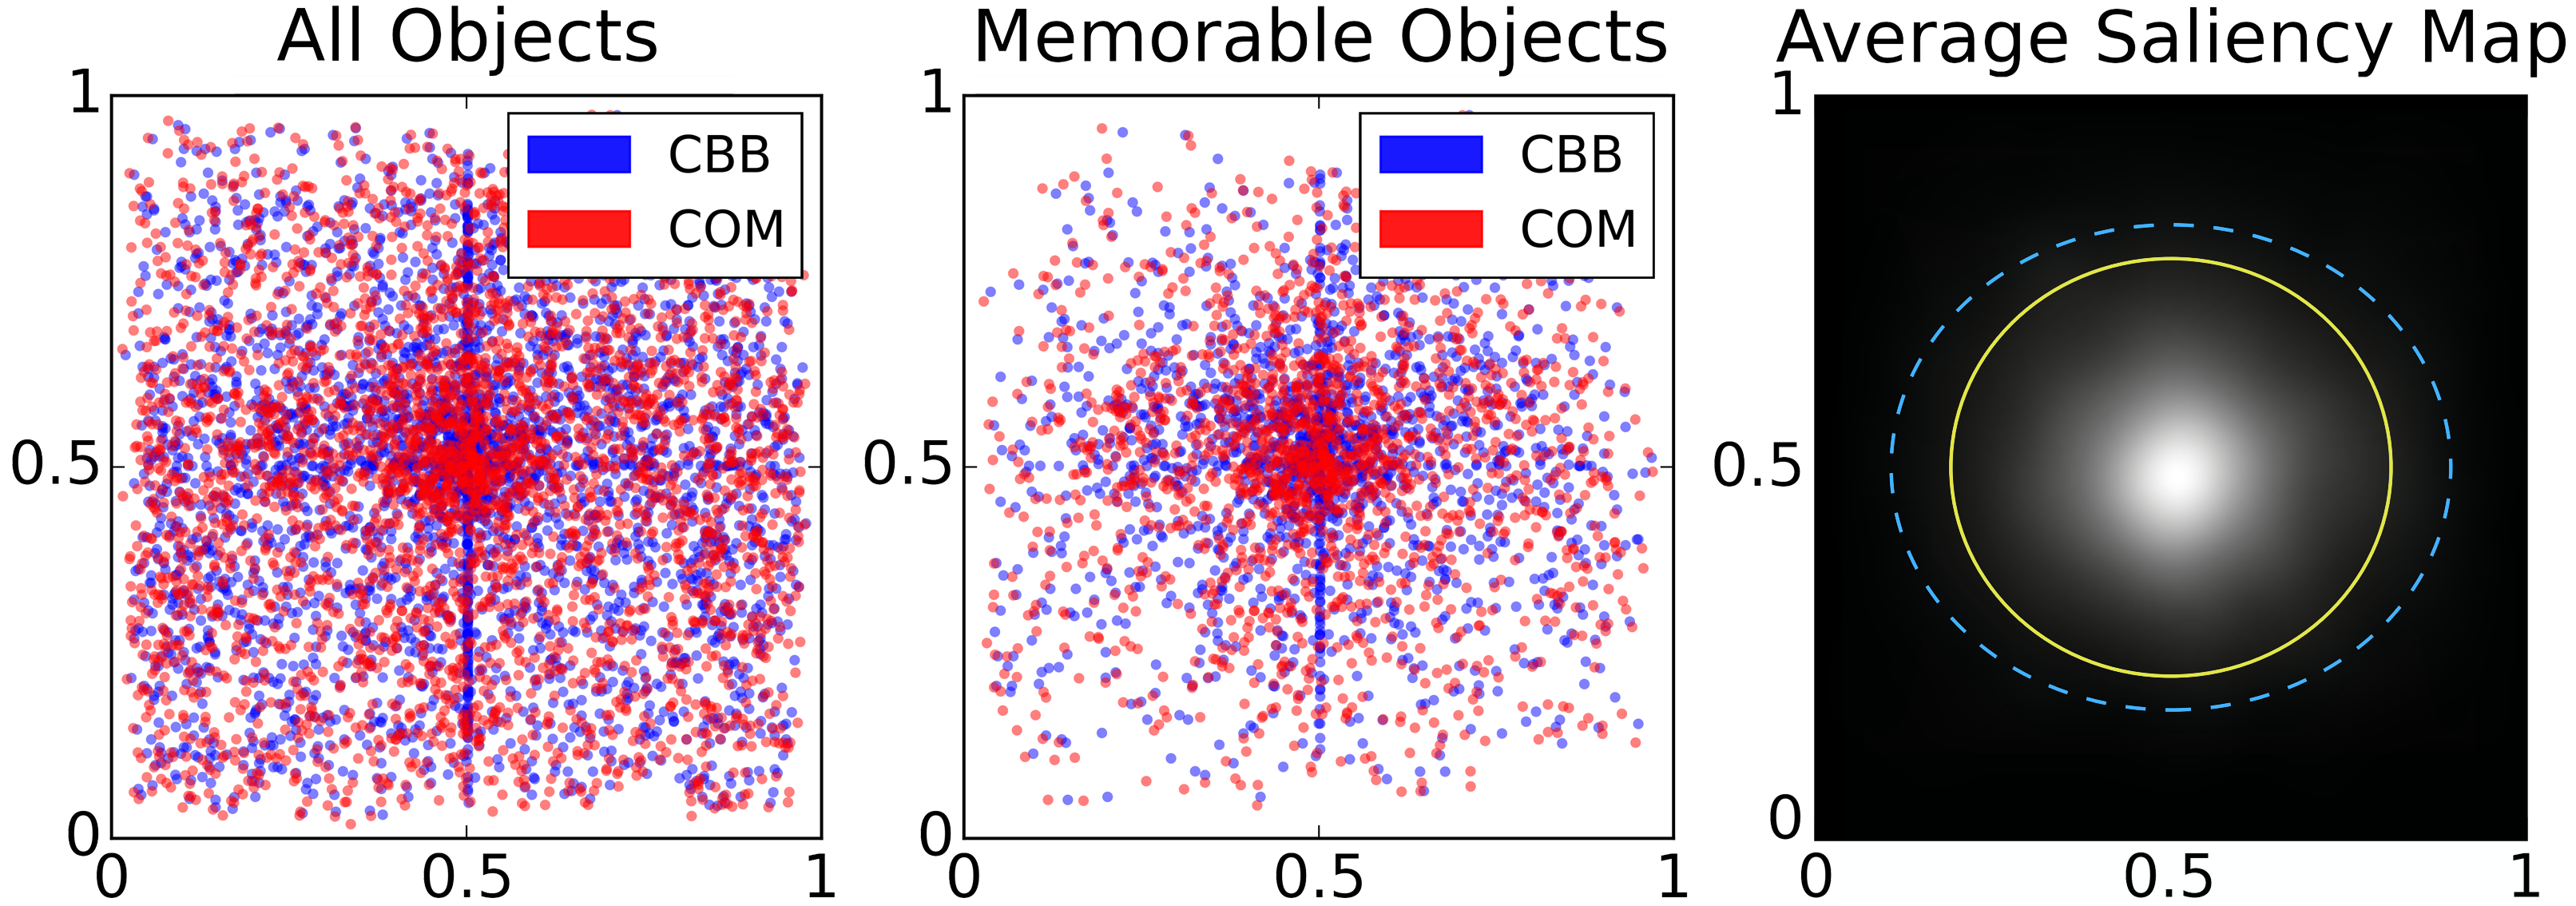
\includegraphics[width=0.47\textwidth]{figures/results/fixation/positions_final2.png}}
\vspace{-5mm}\caption{\footnotesize\textbf{Memorable objects and fixation locations.} Left: Normalized object locations for entire image data set. %xy positions correspond to normalized xy axis.
Both center of object bounding boxes (CBB, blue) and object center of mass (COM, red) are shown. Middle: Locations for memorable objects only. Right: Average ground truth saliency map across the entire dataset. The solid yellow line marks the region with 95\% of all normalized fixation locations. The dashed blue line marks the region with above-median memorable objects. Center bias is more strongly expressed in the fixation locations.}\label{fig:fixPos}
\end{figure}




